\scanpage{112}
\figure{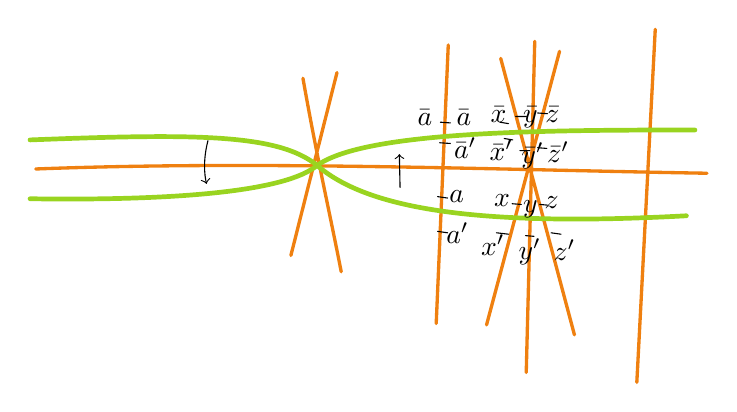
\begin{tikzpicture}[x=.009cm,y=-.009cm,line cap=round,line join=round]
\draw[orange!75!brown,line width=1.2pt] (239,394)..controls(552,382)and(888,395)..(1186,400) (616,266)..controls(636,379)and(653,452)..(670,539) (664,258)--(599,516) (821,219)--(804,612) (895,238)--(999,628) (978,228)--(875,614) (943,214)--(931,681) (1113,197)--(1087,695);
\draw[yellow!60!green,line width=1.7pt] (231,353)..controls(463,344)and(581,344)..(636,389)..controls(702,446)and(845,477)..(1157,460);
\draw[yellow!60!green,line width=1.7pt] (231,436)..controls(443,439)and(593,425)..(636,389)..controls(704,340)and(962,339)..(1169,339);
\draw[->] (482,354)..controls(475,381)and(477,402)..(480,415);\draw[->] (753,420)--(752,373);
\draw (810,328)--(824,329) (809,357)--(824,358) (806,433)--(820,435) (806,482)--(820,484) (894,328)--(906,330) (900,351)--(912,353) (916,320)--(931,320) (947,315)--(961,316) (947,364)--(960,365) (922,368)--(936,368) (911,443)--(924,444) (950,444)--(961,445) (889,484)--(906,486) (930,488)--(942,489) (966,484)--(980,486);
\node at (788,321) {$\deleted{\bar a}$};\node at (843,322) {$\bar a$};\node at (845,365) {$\bar a'$};\node at (833,433) {$a$};\node at (834,485) {$a'$};
\node at (892,317) {$\bar x$};\node at (937,321) {$\bar y$};\node at (968,317) {$\bar z$};\node at (896,368) {$\bar x'$};\node at (940,376) {$\unsure{\bar y'}$};\node at (976,370) {$\bar z'$};
\node at (897,438) {$x$};\node at (937,451) {$\unsure{y}$};\node at (967,442) {$z$};\node at (884,502) {$x'$};\node at (936,511) {$y'$};\node at (985,509) {$z'$};
\end{tikzpicture}}
\figure{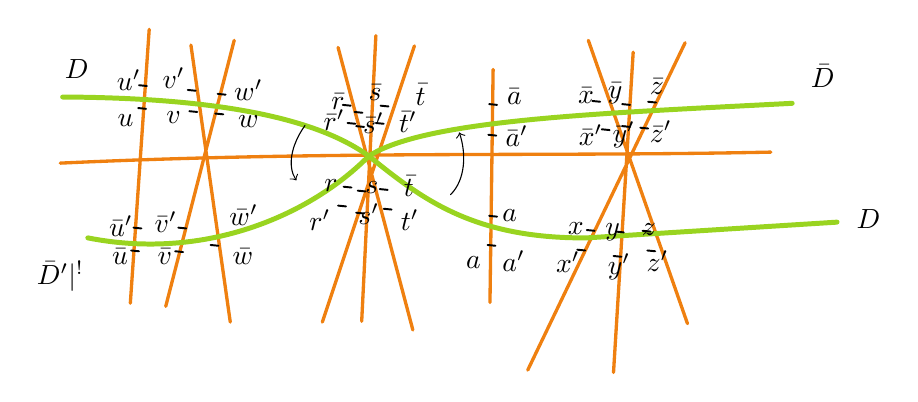
\begin{tikzpicture}[x=.01cm,y=-.01cm,line cap=round,line join=round]
\draw[orange!75!brown,line width=1.2pt] (133,887)..controls(479,871)and(752,879)..(1036,873) (246,717)--(222,1065) (299,737)--(349,1089) (354,731)--(267,1069) (486,740)--(581,1099) (534,725)--(516,1088) (583,738)--(466,1089) (683,768)--(679,1064) (804,731)--(930,1091) (861,746)--(836,1153) (927,734)--(727,1150);
\draw[yellow!60!green,line width=1.8pt] (136,803)..controls(345,804)and(463,833)..(525,878)..controls(591,931)and(656,983)..(802,982)--(1120,962);
\draw[yellow!60!green,line width=1.8pt] (168,982)..controls(320,1012)and(453,951)..(525,878)..controls(597,832)and(812,824)..(1063,811);
\draw[->] (444,839)..controls(425,866)and(422,892)..(433,909);\draw[->] (629,927)..controls(648,908)and(649,875)..(640,848);
\node at (154,768) {$D$};\node at (1102,777) {$\bar D$};\node at (1160,958) {$D$};\node at (133,1031) {$\bar D\unsure{'|^!}$};

\node at (220,781) {$u'$};
\node at (216,833) {$u$};
\node at (210,967) {$\bar u'$};
\node at (209,1006) {$\bar u$};
\node at (277,779) {$v'$};
\node at (277,829) {$v$};
\node at (267,962) {$\bar v'$};
\node at (266,1006) {$\bar v$};
\node at (372,794) {$w'$};
\node at (372,834) {$w$};
\node at (366,953) {$\bar w'$};
\node at (365,1006) {$\bar w$};
\node at (486,809) {$\bar r$};
\node at (481,832) {$\bar r'$};
\node at (533,798) {$\unsure{\bar s}$};
\node at (531,836) {$\unsure{\bar s'}$};
\node at (591,800) {$\bar t$};
\node at (575,835) {$\bar t'$};
\node at (477,915) {$\unsure{r}$};
\node at (463,959) {$r'$};
\node at (529,918) {$\unsure{s}$};
\node at (525,952) {$\unsure{s'}$};
\node at (576,916) {$\bar t$};
\node at (577,959) {$t'$};
\node at (710,802) {$\bar a$};
\node at (713,853) {$\bar a'$};
\node at (704,953) {$a$};
\node at (709,1012) {$a'$};
\node at (658,1013) {$\deleted{a}$};
\node at (801,801) {$\bar x$};
\node at (838,798) {$\bar y$};
\node at (891,790) {$\bar z$};
\node at (807,852) {$\bar x'$};
\node at (849,851) {$\bar y'$};
\node at (896,847) {$\bar z'$};
\node at (788,970) {$x$};
\node at (835,975) {$y$};
\node at (881,971) {$z$};
\node at (778,1013) {$x'$};
\node at (843,1019) {$y'$};
\node at (892,1012) {$z'$};
\draw[line width=.7pt] (233,788)--(243,789);
\draw[line width=.7pt] (232,817)--(242,818);
\draw[line width=.7pt] (226,969)--(236,970);
\draw[line width=.7pt] (223,998)--(233,999);
\draw[line width=.7pt] (295,794)--(305,795);
\draw[line width=.7pt] (297,821)--(307,822);
\draw[line width=.7pt] (283,969)--(293,970);
\draw[line width=.7pt] (279,999)--(289,1000);
\draw[line width=.7pt] (333,799)--(343,800);
\draw[line width=.7pt] (330,824)--(340,825);
\draw[line width=.7pt] (324,991)--(334,992);
\draw[line width=.7pt] (492,813)--(502,814);
\draw[line width=.7pt] (498,836)--(508,837);
\draw[line width=.7pt] (507,822)--(517,823);
\draw[line width=.7pt] (509,840)--(519,841);
\draw[line width=.7pt] (540,814)--(550,815);
\draw[line width=.7pt] (534,836)--(544,837);
\draw[line width=.7pt] (493,917)--(503,918);
\draw[line width=.7pt] (486,941)--(496,942);
\draw[line width=.7pt] (511,922)--(521,923);
\draw[line width=.7pt] (509,950)--(519,951);
\draw[line width=.7pt] (539,920)--(549,921);
\draw[line width=.7pt] (544,945)--(554,946);
\draw[line width=.7pt] (678,812)--(688,813);
\draw[line width=.7pt] (677,851)--(687,852);
\draw[line width=.7pt] (678,954)--(688,955);
\draw[line width=.7pt] (676,991)--(686,992);
\draw[line width=.7pt] (809,808)--(819,809);
\draw[line width=.7pt] (821,844)--(831,845);
\draw[line width=.7pt] (847,812)--(857,813);
\draw[line width=.7pt] (847,840)--(857,841);
\draw[line width=.7pt] (880,809)--(890,810);
\draw[line width=.7pt] (870,842)--(880,843);
\draw[line width=.7pt] (802,972)--(812,973);
\draw[line width=.7pt] (790,997)--(800,998);
\draw[line width=.7pt] (839,974)--(849,975);
\draw[line width=.7pt] (836,1005)--(846,1006);
\draw[line width=.7pt] (873,973)--(883,974);
\draw[line width=.7pt] (879,998)--(889,999);
\end{tikzpicture}}
\uline{NB} $x$ et $\bar x$ (comme $x'$ et $\bar x'$) \unsure{ne sont pas sur le} \unsure{même} \unsure{droite|droites} !
\figure{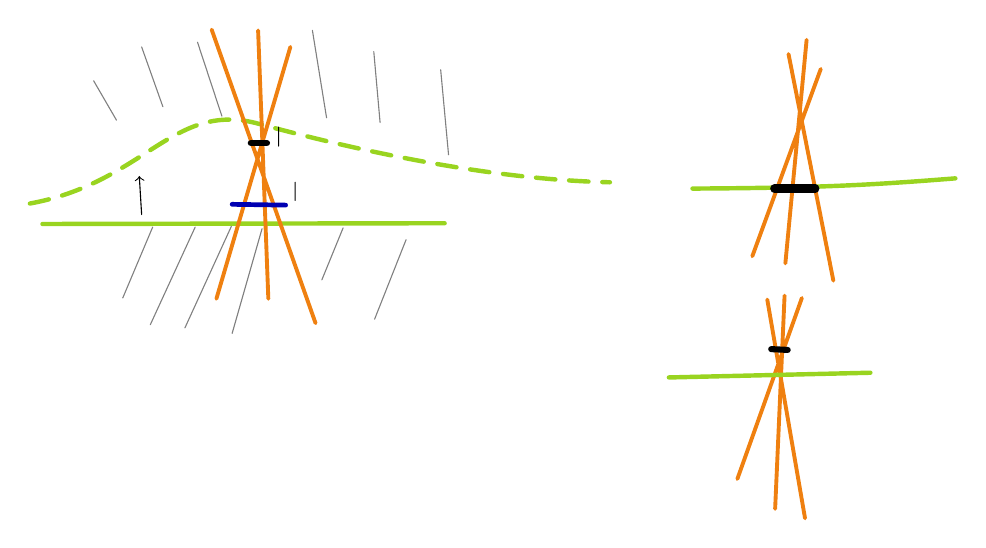
\begin{tikzpicture}[x=.01cm,y=-.01cm,line cap=round,line join=round]
\draw[yellow!60!green,line width=1.6pt] (185,1552)--(696,1551);
\draw[yellow!60!green,line width=1.6pt,dash pattern=on 7pt off 5pt] (169,1526)..controls(316,1499)and(351,1394)..(461,1425)..controls(620,1468)and(774,1496)..(906,1499);
\draw[orange!75!brown,line width=1.4pt] (400,1305)--(532,1678) (459,1306)--(472,1647) (500,1327)--(406,1647);
\draw[line width=2.4pt] (450,1449)--(470,1449);
\draw[blue!70!black,line width=1.7pt] (426,1527)--(494,1528);
\draw[->] (485,1429)--(485,1453) (506,1522)--(506,1499) (311,1540)--(308,1491);
\draw[gray,line width=.4pt] (250,1370)--(279,1420) (311,1327)--(338,1403) (382,1321)--(413,1415) (528,1306)--(546,1417) (606,1333)--(614,1423) (691,1356)--(701,1464) (325,1556)--(287,1646) (379,1556)--(322,1680) (425,1555)--(366,1684) (464,1558)--(426,1691) (567,1557)--(540,1623) (647,1572)--(607,1673);
\draw[orange!75!brown,line width=1.4pt] (1133,1336)--(1190,1624) (1156,1318)--(1129,1602) (1174,1355)--(1087,1593);
\draw[yellow!60!green,line width=1.6pt] (1011,1507)..controls(1170,1506)and(1232,1503)..(1345,1494);
\draw[line width=3pt] (1115,1507)--(1167,1507);
\draw[orange!75!brown,line width=1.4pt] (1106,1648)--(1154,1926) (1128,1643)--(1116,1914) (1150,1646)--(1068,1876);
\draw[yellow!60!green,line width=1.6pt] (981,1747)--(1237,1741);
\draw[line width=2.2pt] (1111,1711)--(1132,1712);
\end{tikzpicture}}
\begin{verbatim}
*******************************************************************************
*JESNEWS DU 09/08/1982 C68 CADARACHE                                          *
*******************************************************************************
*      DEPUIS LE 1/7/82 LES ALIAS DES COMMANDES LIBRARIAN                     *
*             LIBGET (LG) ET LIBSAVE (LS) SONT SUPPRIMES,                     *
*             POUR EVITER UNE POSSIBILITE DE CONFLIT AVEC                     *
*             LE MEME ALIAS DES COMMANDES STANDARD IBM.                       *
*      ********                                                               *
* ATTENTION                                                                   *
*   MISE EN SERVICE LE VENDREDI 30/7/82 A 8H00 DE LA DEUXIEME PHASE DE GAF    *
*     SUR 168 CADARACHE.                                                      *
*     ELLE PERMET D'UTILISER DANS LA CDE. KEEP TSO ET DANS LA PROCEDURE KEEP  *
*     BATCH UNE POSSIBILITE D'AFFECTATION DE TYPE DE SAUVEGARDE AU NIVEAU DU  *
*     FICHIER.CETTE POSSIBILITE EST VIVEMENT CONSEILLEE.                      *
*     POUR PLUS AMPLES INFORMATIONS VOIR NOTE TECHNIQUE CISI MVS140,LA NOTE   *
*     MVS 143 ETANT SUPPRIMEE.                                                *
*                                                                             *
* EXEMPLES D'UTILISATION:                                                     *
*                                                                             *
*  BATCH:  DSN=NOM.DU.FICHIER.A.SAUVEGARDER,DELAY=TYPE DE SAUVEGARDE          *
*                                                                             *
*  TSO:                                                                       *
*  K DA('NOM DU FICHIER A SAUVEGARDER') DELAY(TYPE DE SAUVEGARDE)             *
*                                                                             *
*  TYPES DE SAUVEGARDE:                                                       *
*                                                                             *
*      W       SAUVEGARDE HEBDO.                                              *
*      D       SAUVEGARDE JOURNALIERE.                                        *
*      NOS     SAUVEGARDE MENSUELLE.                                          *
*      W       PARAMETRE PAR DEFAUT.                                          *
*                                                                             *
*******************************************************************************
******************************************************************
*                                                                *
*                  - J E S N E W S   F R 1 -      LE 16/08/82    *
*                                                                *
*----------------------------------------------------------------*
*                                                                *
*  DEPUIS LE LUNDI 12 JUILLET 82, LES CLASSES DE TRAVAUX D ET E  *
*  SERONT ETENDUES POUR UNE TAILLE MEMOIRE SUPERIEURE A 1024 K   *
*  SE REPORTER A LA NOTE TECHNIQUE MVS141.                       *
*                                                                *
*----------------------------------------------------------------*
*  A PARTIR DU LUNDI 9 AOUT 1982 , IL SERA POSSIBLE D'IMPRIMER   *
*  SUR XEROX 9700 (DESTINATION SAC) DES FICHIERS UTILISANT LE    *
*  COUPLE DE JEUX DE CARACTERES : (GS15,GT15)                    *
*                                                                *
*----------------------------------------------------------------*
*                                                                *
*-LE 15/08/82 :                                                  *
*-------------                                                   *
*  -LE 370/168 SERA ARRETE DU VENDREDI 20 AOUT A 19H JUSQU'AU    *
*   LUNDI 23 AOUT A 8H.( MISE A NIVEAU TECHNIQUE.).              *
*                                                                *
******************************************************************
\end{verbatim}
\margin{111}
